\documentclass[a4paper, 10.5pt, oneside, openany, uplatex]{jsarticle}

\author{山内 仁喬}
% 余白の設定.
% 参考文献:Latex2e 美文書作成入門, 14.3ページレイアウトの変更

% 行長の変更
\setlength{\textwidth}{40zw}           %全角40文字分

% 行間を制御するコマンド
\renewcommand{\baselinestretch}{0.9}

% 左マージンを変更
\setlength{\oddsidemargin}{25truemm}   % 左余白
\addtolength{\oddsidemargin}{-1truein} % 左位置デフォルトから-1inch

% 上マージンを変更
\setlength{\topmargin}{15truemm}       % 上余白
\addtolength{\topmargin}{-1truein}     % 上位置デフォルトから-1inch

% 本文領域の縦横の長さ変更
\setlength{\textheight}{242truemm}     % テキスト高さ: 297-(25+30)=242mm
\setlength{\textwidth}{160truemm}      % テキスト幅:  210-(25+25)=160mm
\setlength{\fullwidth}{\textwidth}     % ページ全体の幅


% 図・表の個数などの設定.
%% 図・表を入りやすさを制御するパラメーター
\setcounter{topnumber}{4}
\setcounter{bottomnumber}{4}
\setcounter{totalnumber}{4}
\setcounter{dbltopnumber}{3}
\setcounter{tocdepth}{1} % 項レベルまで目次に反映させるコマンド.
\renewcommand{\topfraction}{.95}
\renewcommand{\bottomfraction}{.90}
\renewcommand{\textfraction}{.05}
\renewcommand{\floatpagefraction}{.95}

% 使用するパッケージを記述.
\usepackage{amsmath} % 複雑な数式を使うときに便利
\usepackage{dcolumn}
\usepackage{color}
\usepackage{tabularx, dcolumn}
\usepackage{bm} % 数式環境内で太字を使うときに便利.
\usepackage{subcaption}  % 関連した複数の図を並べる時に使う
\usepackage[dvipdfmx]{graphicx} % 画像を挿入したり,テキストや図の拡大縮小・回転を行う.
\usepackage{verbatim} % 入力どおりの出力を行う.
\usepackage{makeidx} % 索引を作成できる.
\usepackage{dcolumn} % 表の数値を小数点で桁を揃える.
\usepackage{lscape} % 図表を90度横に倒して配置する.
\usepackage{setspace} % 行間調整.

\def\mbf#1{\mbox{\boldmath ${#1}$}}

% \newcolumntype{d}{D{+}{\,\pm\,}{4,5}}
% \newcolumntype{i}{D{+}{\,\pm\,}{-1}}
% \newcolumntype{.}{D{.}{.}{6,3}}

\begin{document}


\title{分子モデリング}
\maketitle

\section{濃度換算}
分子モデリングをする際には, 実験で使用されたイオン濃度をシミュレーションでも再現することが多い. 
その際に, 何個のイオン原子を含めるかを計算する必要がある. 
この章では, 濃度換算についてまとめる. 


\subsection{モル濃度}

モル濃度の定義は以下の通りである. 
\begin{itemize}
    \item 単位体積の溶液中の溶質の物質量
    \item SI単位系で $\mathrm{mol}/\mathrm{m}^{3}$
\end{itemize}

モル濃度をモーラー($\mathrm{M} = \mathrm{mol}/\mathrm{L}$)へ単位変換は以下の通りである. 
\begin{align}
    \mathrm{mol}/\mathrm{m}^{3} =&
    10^{-3} ~\mathrm{mol} / \mathrm{dm}^{3} \\ =&
    10^{-3} ~\mathrm{mol} / \mathrm{L} \\ =&
    10^{-3} ~\mathrm{M} \\ =&
    1 ~\mathrm{mM}
\end{align}


\subsubsection{例1: $2.00~\mathrm{mol/L}$のNaCl水溶液を100~mL調整する}
NaClのモル濃度は58.4~g/molである. 
必要なNaClは
\begin{align}
    &2.00~(\mathrm{mol/L}) \times 58.4~(\mathrm{g/mol}) = 116.8~(\mathrm{g/L}) \\
    &116.8~(\mathrm{g/L}) = 0.1168~(\mathrm{g/}10^{-3}\mathrm{L}) = 0.1168~(\mathrm{g/mL}) \\
    &0.1168~(\mathrm{g/mL}) \times 100~(\mathrm{mL}) = 11.7 (\mathrm{g})
\end{align}
故に11.7~gのNaClを100mLになるまで水を足せば, 2.00~mol/LのNaCl水溶液が完成する. 


\subsubsection{例2: NaCl水溶液におけるNaClの質量分率, 体積, モル濃度の計算}

100~mLの水に11.6~gのNaClが溶解している. 溶液の密度は1.07~g/mL, 
水の密度を1.00~g/mLとする. この時, NaClの質量分率は
\begin{equation}
    \frac{11.6~(\mathrm{g})}{11.6~(\mathrm{g}) + 100~(\mathrm{g})}
    \times
    100 \%
    =
    10.5 \%
\end{equation}
一方で水(H$_2$O)の質量分率は
\begin{equation}
    \frac{100~(\mathrm{g})}{11.6~(\mathrm{g}) + 100~(\mathrm{g})}
    \times
    100 \%
    =
    89.6 \%
\end{equation}
である. 溶液の密度から溶液の体積は, 
\begin{equation}
    \frac{11.6~(\mathrm{g}) + 100~(\mathrm{g})}{1.07~(\mathrm{g/mL})}
    =
    104~(\mathrm{mL})
\end{equation}
NaClのモル濃度は
\begin{equation}
    11.6~(\mathrm{g}) \times
    \frac{1}{58.4~(\mathrm{g/mol})} \times
    \frac{1}{104~(\mathrm{mL})} \times
    1000 =
    1.91~\mathrm{M}
\end{equation}


\subsubsection{例3: 水溶液に含まれているイオンの数を換算する}

一辺100~{\AA}の箱にNaClが150~mM = 150 mol/m$^3$入っているとする. 
この時に, NaClがいくつ含まれているかを数える. 
まず体積をSI単位系で表す. 
\begin{equation}
    100~\mathrm{\AA} =
    100 \times 10^{-10}~\mathrm{m} =
    10^{-8}~\mathrm{m}
\end{equation}
だから, 
\begin{equation}
    (100~\mathrm{\AA})^3 =
    (10^{-8}~\mathrm{m})^3 =
    10^{-24}~\mathrm{m}^3
\end{equation}
150 mol/m$^3$の濃度の時, 1立方メートルあたりに含まれるNaClのイオンの数は, 
\begin{align}
    150 ~(\mathrm{mol/}\mathrm{m}^3) &=
    150 \times 6.0 \times 10^{23} ~(\mathrm{m}^{-3}) \\ &=
    900 \times 10^{23}  ~(\mathrm{m}^{-3}) \\ &=
    9 \times 10^{25} ~(\mathrm{m}^{-3})
\end{align}
したがって, 一辺が100~{\AA}の箱に含まれるNaClの数は, 
\begin{equation}
    9 \times 10^{25}~(\mathrm{m}^{-3}) \times 10^{-24} ~(\mathrm{m}^3)
    = 90
\end{equation}
と計算される. つまり, 90個のNaClが含まれている. 


\subsubsection{例4: 体積が$V$~({\AA}$^3$)の箱にモル濃度$x$~mMのNaClを入れる}

単位をmMからmol/m$^3$に変換すると, 
\begin{equation}
    x~(\mathrm{mM}) = x ~(\mathrm{mol/m}^{3})
\end{equation}
体積の単位をSI単位系に直すと, 
\begin{equation}
    V~(\mathrm{\AA}^{3}) =
    V \times 10^{-30} ~(\mathrm{m}^3)
\end{equation}
したがって, 
\begin{align}
    x~(\mathrm{mM}) &=
    x~(\mathrm{mol/m}^3) \\ &=
    x \times 6.022 \times 10^{23} ~(\mathrm{mol}^{-1})(\mathrm{mol/m}^3) \\ &=
    x \times 6.022 \times 10^{23} ~(\mathrm{m}^{-3}) \\ &=
    6.022 x \times 10^{23} ~(\mathrm{m}^{-3})
\end{align}

よって, 体積が$V$~({\AA}$^3$)の箱に含まれるイオンの数は, 
\begin{align}
    6.022 x \times 10^{23} \times V \times 10^{-30} =
    6.022 x V \times 10^{-7} (\mathrm{個})
\end{align}
と計算される. 

\clearpage
\section{水の初期配置について}
常温常圧における水の密度に合わせて水を配置するには, どのような間隔で並べればいいかを考える. 
水の質量, 常温常圧での密度は
\begin{itemize}
    \item 水の質量 = $18~(\mathrm{g/mol})$
    \item 水の密度 = $998.233~(\mathrm{kg/m}^3) \simeq 1.0~(\mathrm{g/cm}^3)$
    \item アボガドロ定数 = $6.02214086 \times 10^{23} ~(\mathrm{mol}^{-1})$
\end{itemize}
である. 
$1~\mathrm{cm} = 1.0 \times 10^{8}~{\mathrm{\AA}}$であるので, 
\begin{align}
    1.0~(\mathrm{g/cm}^{3}) &=
    \frac{6.02214086 \times 10^{23}}{18} ~(\mathrm{cm}^{-3}) \\ &=
    \frac{6.02214086 \times 10^{23}}{18} \times \frac{1}{10^{24}}
    ~(\mathrm{\AA}^{-3}) \\ &=
    0.334 \times \frac{1}{10} ~(\mathrm{\AA}^{-3}) \\ &=
    0.0334 ~(\mathrm{\AA}^{-3})
\end{align}
すなわち, 1~{\AA}$^3$に0.0334個の水分子が存在するような密度であるので, 1~{\AA}に0.3220個の間隔で水分子を置けばよいという計算となる. 
よって, 3.104~{\AA}に1個の水を置けば良い. 


\section{一般化螺旋集合 (GSS: Generalized Spiral Set)}
ミセルの初期構造を配置するなど, 任意の点数を球面上にできるだけ等間隔にプロットするためのアルゴリズムを考える. 
これを実現する一つの方法として, 螺旋を球面状に射影することが挙げられる. 
このような点の集合を一般化螺旋集合という. 

\subsection{アルゴリズム}
区間$[-1,~1]$を$(N-1)$等分した離散パラメータ$h$は自然数$0\le k \le N-1$を用いれば, 
\begin{equation}
    h_{k} = -1 + 2 \frac{k}{N-1}
\end{equation}
と書くことができる. 
一般化螺旋集合は以下のような漸化式で表される偏角を持つような点の集合である. 
\begin{align}
    \theta_{k} &= \arccos(h_{k}) \\
    \phi_{0} &= 0 \\
    \phi_{k+1} &= \phi_{k} + \frac{3.6}{\sqrt{N}} \frac{1}{\sqrt{1-h_{k^{2}}}}
\end{align}
$h_{k} = \pm 1$, つまり$k=0,~N-1$のとき$\phi_{k+1}$が発散してしまうのに注意. 

\clearpage

\section{RESPAC: 粗視化粒子に小数電荷を割り当てるアルゴリズム}
粗視化モデルを使用した場合, 分子の持つ電荷は粗視化粒子の座標点に置かれることがあるが、
このような電荷の置き方はしばしば適切ではない.
例えば, アミノ酸1残基を1粒子に粗視化して粒子の代表点をC$_\alpha$原子上に定めた場合, $+1$, $0$, $-1$の電荷をC$_\alpha$原子上に置くことになる. しかし、荷電アミノ酸は側鎖の先端に電荷を持っているため, C$_\alpha$原子上に$+1$, $0$, $-1$の電荷を置く取り扱いは, 実際の分子描像と解離がある.
このような問題点を解決するためのアルゴリズムとして\textbf{RESPAC}~\cite{Terakawa2014}が提案されている.
RESPACでは全原子レベルの部分電荷によって計算された静電ポテンシャルを再現するように粗視化粒子の部分電荷を決定する.
量子化学計算で得られた静電ポテンシャルを再現するように全原子の部分電荷を決定するアルゴリズムRESP~\cite{Bayly1993, Besler1990}に由来して, RESPACと名前がつけられている.

\subsection{RESPACの流れ}
RESPACの一連の流れは次の通りである:
\begin{enumerate}
    \item 全原子モデルに対して部分電荷を割り当てる(\texttt{PDB2PQR})
    \item 全原子の部分電荷に基づいて静電ポテンシャルを計算する(\texttt{APBS})
    \item 粗視化構造について, 蛋白質表面のアミノ酸残基を特定する(\texttt{surface})
    \item 蛋白質表面のアミノ酸残基について, 全原子モデルから得られた静電ポテンシャルを再現するように, 最適な粗視化粒子の部分電荷を決定する(\texttt{pdc})
\end{enumerate}

\subsection{RESPACの理論}
\subsubsection{全原子モデルの部分電荷が作り出す静電ポテンシャルを計算する}
連続誘電体モデルにおいて、全原子モデルの部分電荷が作り出す静電ポテンシャル$\phi_{\mathrm{ref}}$はPoisson–Boltzmann方程式
\begin{equation}
    \nabla \cdot
    \left[
        \epsilon(\bm{r}) \nabla \cdot \phi_{\mathrm{ref}}(\bm{r})
    \right]
    -
    \epsilon(\bm{r}) \kappa \sinh[\phi_{\mathrm{ref}}(\bm{r})]
    +
    \frac{4 \pi \rho(\bm{r})}{k_{\mathrm{B}}T}
    =
    0
\end{equation}
を解くことで得られる.
ここで, $\bm{r}$は分子の周りのグリッド点の位置ベクトル、$\epsilon(\bm{r})$は位置に依存した誘電率、$\kappa$はデバイ長の逆数、$\rho(\bm{r})$は原子電荷密度, $k_{\mathrm{B}}$はボルツマン定数,
$T$は温度である.

\subsubsection{粗視化粒子が作り出す静電ポテンシャル}
Debye--H\"{u}ckel近似を適用している場合, 粗視化粒子による静電ポテンシャルは
\begin{equation}
    \phi(\bm{r})
    =
    \sum_{i=1}^{N}
    q_{i}
    \frac{\exp(-\kappa |\bm{r} - \bm{r}_{i}|)}{\epsilon |\bm{r} - \bm{r}_{i}|}
\end{equation}
と計算できる.
ここで$\bm{r}_{i}$は粗視化粒子の位置ベクトル, $\epsilon$は溶媒の誘電率である.

\subsubsection{粗視化粒子の部分電荷の決定}
粗視化粒子の部分電荷は次の評価関数が最小となるように決定する:
\begin{equation}
    \mathcal{L} (\phi_{\mathrm{ref}}^{\mathrm{PB}}, \bm{q})
    =
    \int_{\Omega} d\bm{r}
    \left[
        \phi_{\mathrm{ref}}^{\mathrm{PB}}
        -
        \sum_{i=1}^{N}
        q_{i}
        \frac{\exp(-\kappa |\bm{r} - \bm{r}_{i}|)}{\epsilon |\bm{r} - \bm{r}_{i}|}
    \right]^{2}
    +
    \delta \sum_{i=1}^{N} (q_{i} - q_{i}^{\prime})^{2}
    +
    \lambda(q_{\mathrm{tot}} - \sum_{i=1}^{N} q_{i})^{2}
    \label{Eq:RESPAC-Evaluation-Function}
\end{equation}
ここで, $\Omega$は分子に近接する空間を表す. また$\phi_{\mathrm{ref}}^{\mathrm{PB}}$は全原子モデルから計算されて参照静電ポテンシャル, $\bm{q}$は粗視化粒子の電荷の集合を表す. $q_{i}^{\prime}$はターゲット電荷, $q_{\mathrm{tot}}$は分子の総電荷量である.
$\delta$, $\lambda$はラグランジュの未定乗数である.

評価関数の第1項目は全原子から求めた参照静電ポテンシャルが粗視化粒子が形成する静電ポテンシャルと一致することを要請する束縛条件である.
第2項目は各粗視化粒子の部分電荷に対する束縛条件である. この条件はRESP論文において部分電荷のオーバーフィッティングを避けるために導入された束縛条件である. 特に理由がなければRESP論文で述べられているように$q_{i}^{\prime} = 0$と設定することが多い.
第3項目は分子の総電荷量を固定するための束縛条件である.

続いて評価関数が極値を取る条件から粗視化粒子の部分電荷計算する方法を見ていく.
実際の計算では離散化していた方が便利なので, 評価関数(\ref{Eq:RESPAC-Evaluation-Function})の積分を和で置き換える:
\begin{equation}
    \mathcal{L} (\phi_{\mathrm{ref}}^{\mathrm{PB}}, \bm{q})
    =
    \sum_{i=1}^{M}
    \left[
        \phi_{i}^{\mathrm{PB}}
        -
        \sum_{j=1}^{N}
        q_{j}
        \frac{\exp(-\kappa |\bm{r} - \bm{r}_{j}|)}{\epsilon |\bm{r} - \bm{r}_{j}|}
    \right]^{2}
    +
    \delta \sum_{j=1}^{N} (q_{j} - q_{j}^{\prime})^{2}
    +
    \lambda(q_{\mathrm{tot}} - \sum_{j=1}^{N} q_{j})^{2}
    \label{Eq:RESPAC-Evaluation-Function-Discrete}
\end{equation}
ここで$i$はグリッド点, $j$は粗視化粒子のインデックスを表していることに注意すること.
評価関数が極値を取る条件
\begin{equation}
    \frac{\partial \mathcal{L}}{\partial q_{k}} = 0
\end{equation}
より
\begin{equation}
    \sum_{i=1}^{M}
    2
    \left[
        \phi_{i}^{\mathrm{PB}}
        -
        \sum_{j=1}^{N}
        q_{j}
        \frac{\exp(-\kappa r_{ij})}{\epsilon r_{ij}}
    \right]
    \frac{\exp(-\kappa r_{ik})}{\epsilon r_{ik}}
    +
    2 \delta \sum_{j=1}^{N} (q_{j} - q_{j}^{\prime})
    +
    2 \lambda(q_{\mathrm{tot}} - \sum_{j=1}^{N} q_{j})
    =
    0
\end{equation}
を得る. これを整理すると,
\begin{equation}
    \sum_{i=1}^{M} \sum_{j=1}^{N}
    \left\{
        \frac{\exp[-\kappa (r_{ij} + r_{ik})]}{\epsilon^{2} r_{ij}r_{ik}}
        -
        \lambda
    \right\} q_{j}
    -
    \delta q_{k}
    =
    \sum_{i=1}^{M}
    \frac{\exp(-\kappa r_{ik})}{\epsilon r_{ik}} \phi_{i}^{\mathrm{PB}}
    -
    \delta q_{k}^{\prime}
    -
    \lambda q_{\mathrm{tot}}
\end{equation}
となる. 全ての粒子の電荷$q_{k},~k = 1,\ldots,N$について同様の方程式を得ることができるので, 行列形式で書き直すと
\begin{align}
    A_{jk}
    &=
    \sum_{i=1}^{M}
    \frac{\exp[-\kappa(r_{ij} + r_{ik})]}{\epsilon r_{ij}r_{ik}}
    + \lambda^{\prime}
    &&(j\neq k)
    \\
    A_{kk}
    &=
    \sum_{i=1}^{M}
    \frac{\exp[-2\kappa r_{ik}]}{\epsilon r_{ik}^{2}}
    + \delta^{\prime}
    + \lambda^{\prime}
    &&(j = k)
    \\
    B_{j}
    &=
    \sum_{i=1}^{M}
    \frac{\exp[-\kappa r_{ik}]}{\epsilon r_{ik}} \phi_{i}^{\mathrm{PB}}
    +
    \delta^{\prime} q_{k}^{\prime}
    +
    \lambda^{\prime} q_{\mathrm{tot}}
\end{align}
を導入すると
\begin{equation}
    \bm{A} \bm{q} = \bm{B}
\end{equation}
の連立方程式が得られ,
\begin{equation}
    \bm{q} = \bm{A}^{-1}\bm{B}
\end{equation}
のように連立方程式を解くことで最適な部分電荷の値を得ることができる.
なお, 途中で数式の便利のために$\lambda^{\prime} = -\lambda$, $\delta^{\prime} = -\delta$のように置き直した.

\subsubsection{スケーリング係数$\delta$と$\lambda$の決定方法}
評価関数(\ref{Eq:RESPAC-Evaluation-Function})を最小化するためには, 適切なスケーリング係数$\delta$, $\lambda$を選択する必要がある.
分子の総電荷に対する束縛条件のスケーリング係数である$\lambda$は, 得られる有効電荷にあまり影響しないため, 十分大きい値を設定しておけばいい. 例えばRESPAC論文では$\lambda = 10^{5}$と設定している.

一方で, 各粒子に対する参照電荷の束縛条件のスケーリング係数$\delta$の値はRESPACで得られる有効電荷に大きく影響を与える.
最適な$\delta$の値を得るためのプロトコルとして次のようなものが提案されている:
(i) 全原子モデルに基づいた短いMDシミュレーションを実行して, 10個の構造をサンプリングする.
(ii) 各構造に対して、評価関数(\ref{Eq:RESPAC-Evaluation-Function})を最小化するようにして粗視化電荷を決定する.
(iii) 得られた粗視化電荷$\bm{q}$に対して, 規格化された誤差$\Delta (\bm{q}(\delta))$
\begin{equation}
    \Delta (\bm{q}(\delta))
    =
    \frac
    {\int_{\Omega} d\bm{r}
        \left[
            \phi_{\mathrm{ref}}^{\mathrm{PB}}
            -
            \sum_{i}^{N} q_{i}
            \frac{\exp(-\kappa |\bm{r} - \bm{r}_{i}|)}{\epsilon |\bm{r} - \bm{r}_{i}|}
        \right]^{2}
    }
    {
        \int_{\Omega} d\bm{r}[\phi_{\mathrm{ref}}^{\mathrm{PB}}]^{2}
    }
\end{equation}
を計算する.
(iv) サンプリングした10個の構造に対して誤差の平均$\langle \Delta (\bm{q}(\delta)) \rangle$を計算し, 誤差の平均が最小となるような$\delta$を採用する.

%\section{水のモデル}


%\subsection{Sub section}

% \subsubsection{Sub sub section}
% \begin{figure}
%  \begin{center}
%   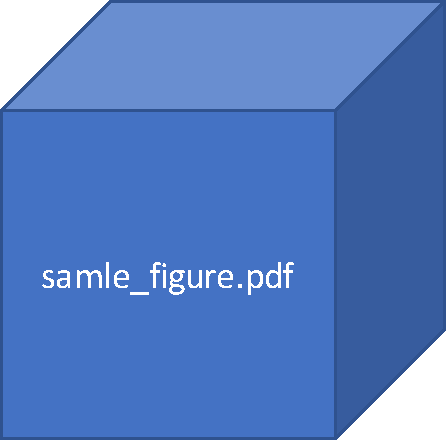
\includegraphics[width=0.5\hsize]{../figure/sample/sample_figure.pdf}
%   \caption{This is caption of sample figure.}
%   \label{Fig:Sample}
%  \end{center}
% \end{figure}

% \paragraph{Paragraph}

\bibliographystyle{junsrt}
\bibliography{modeling-molecules}
\end{document}

